\documentclass{standalone}
\usepackage{tikz}
\usetikzlibrary{patterns, positioning}
\usepackage[sfdefault]{ClearSans} %% option 'sfdefault' activates Clear Sans as the default text font
\usepackage[T1]{fontenc}

\begin{document}
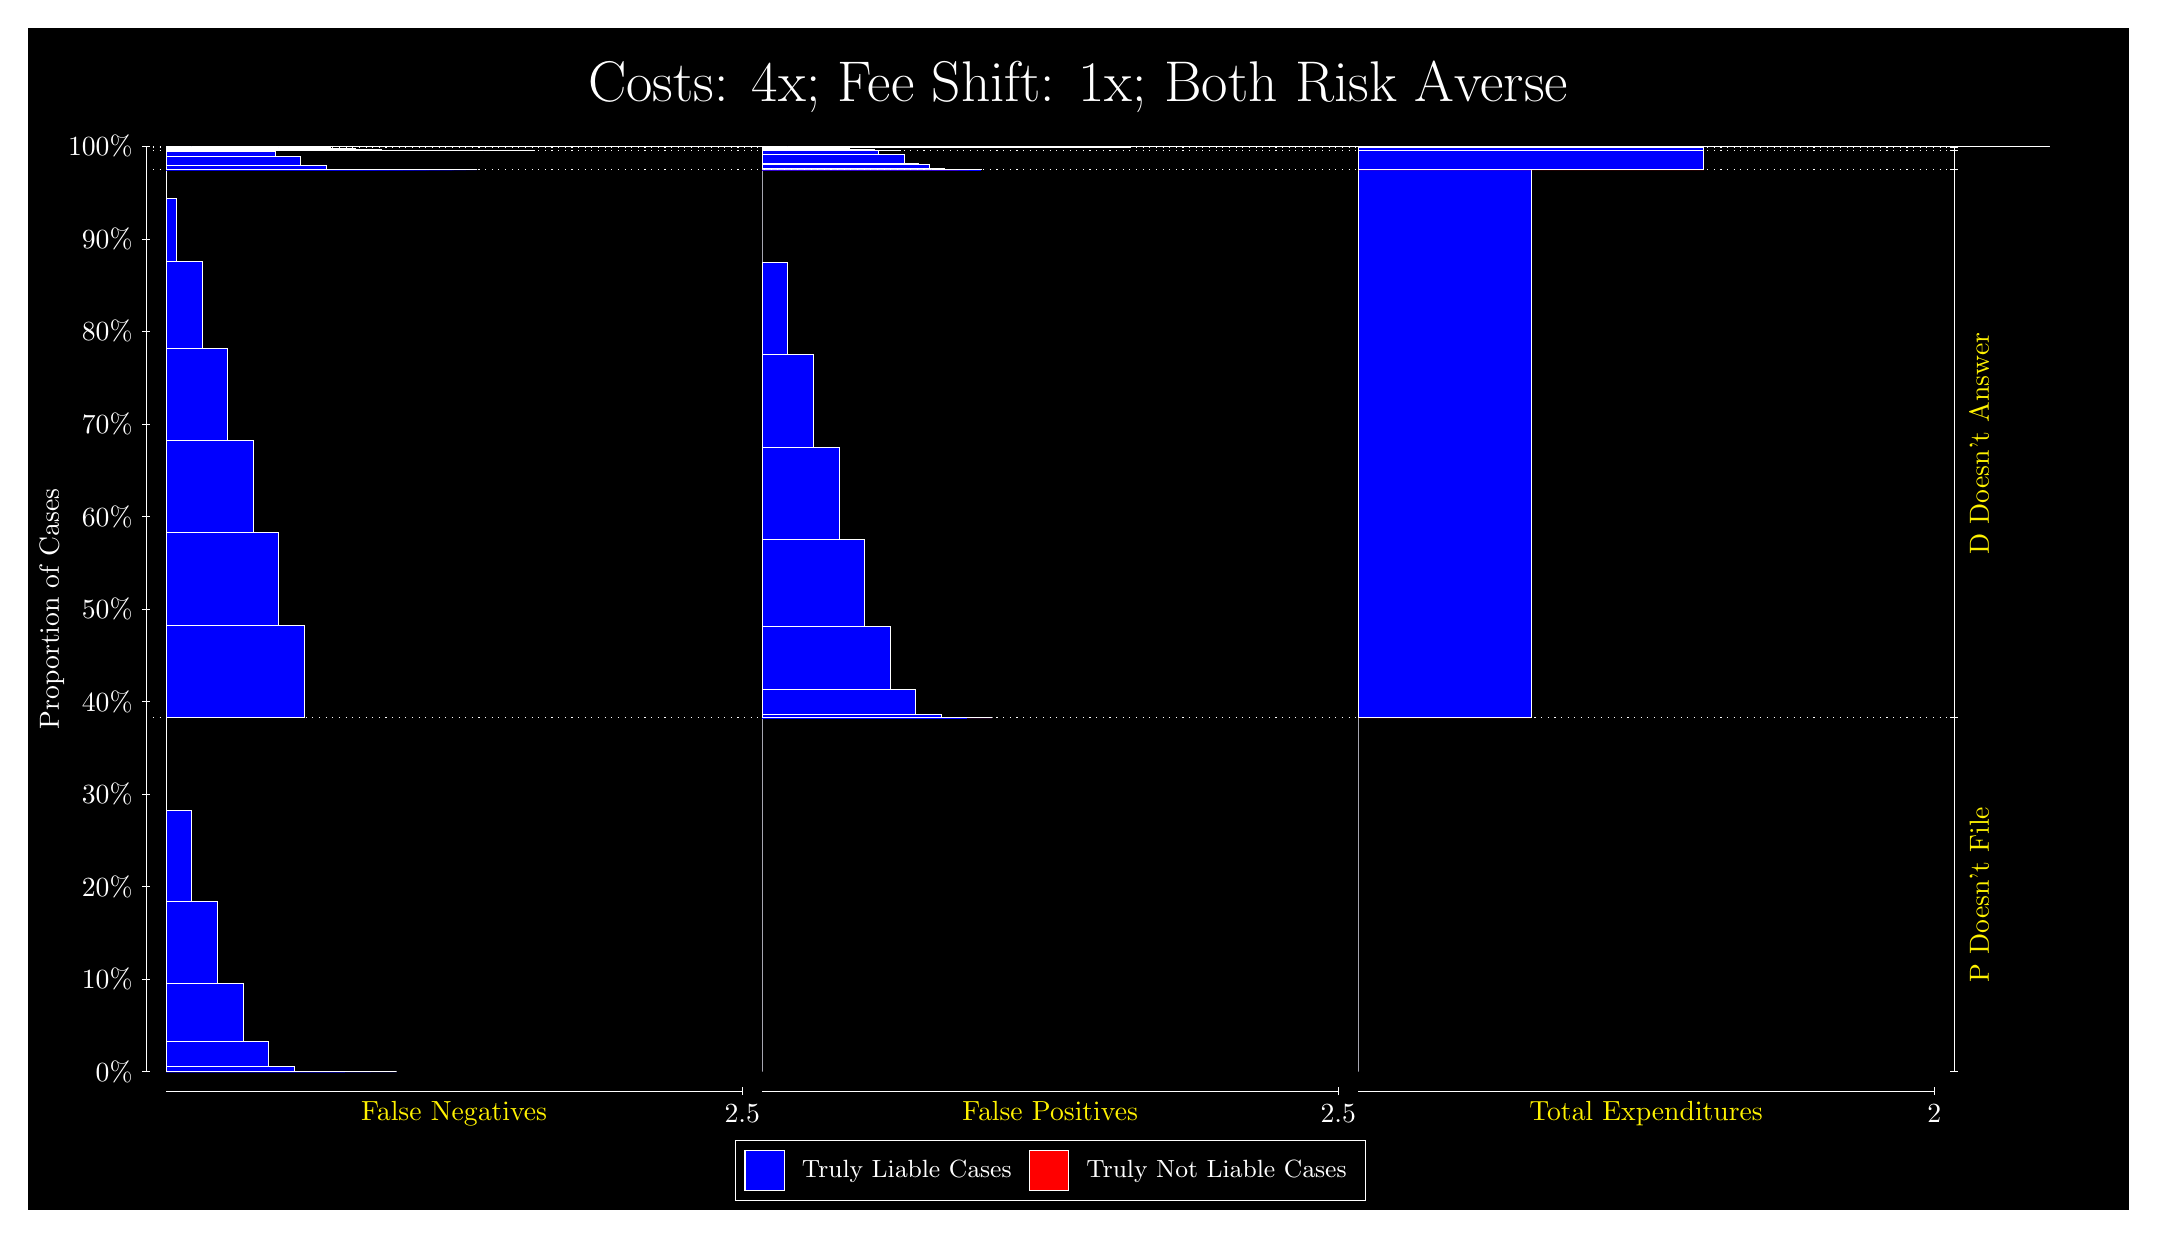
\begin{tikzpicture}
\draw[fill=black] (0,0) rectangle (26.667,15);
\draw[text=white] (0,13.5) rectangle (26.667,15) node[midway] {\huge Costs: 4x; Fee Shift: 1x; Both Risk Averse};
\draw[white, very thin] (1.5,1.75) -- (1.5,13.5);
\node[rotate=90, text=white, anchor=center] at (0.3, 7.625) {Proportion of Cases};
\draw[white, very thin] (1.45,1.75) -- (1.55,1.75);
\node[text=white, anchor=east] at (1.45, 1.75) {0\%};
\draw[white, very thin] (1.45,2.925) -- (1.55,2.925);
\node[text=white, anchor=east] at (1.45, 2.925) {10\%};
\draw[white, very thin] (1.45,4.1) -- (1.55,4.1);
\node[text=white, anchor=east] at (1.45, 4.1) {20\%};
\draw[white, very thin] (1.45,5.275) -- (1.55,5.275);
\node[text=white, anchor=east] at (1.45, 5.275) {30\%};
\draw[white, very thin] (1.45,6.45) -- (1.55,6.45);
\node[text=white, anchor=east] at (1.45, 6.45) {40\%};
\draw[white, very thin] (1.45,7.625) -- (1.55,7.625);
\node[text=white, anchor=east] at (1.45, 7.625) {50\%};
\draw[white, very thin] (1.45,8.8) -- (1.55,8.8);
\node[text=white, anchor=east] at (1.45, 8.8) {60\%};
\draw[white, very thin] (1.45,9.975) -- (1.55,9.975);
\node[text=white, anchor=east] at (1.45, 9.975) {70\%};
\draw[white, very thin] (1.45,11.15) -- (1.55,11.15);
\node[text=white, anchor=east] at (1.45, 11.15) {80\%};
\draw[white, very thin] (1.45,12.325) -- (1.55,12.325);
\node[text=white, anchor=east] at (1.45, 12.325) {90\%};
\draw[white, very thin] (1.45,13.5) -- (1.55,13.5);
\node[text=white, anchor=east] at (1.45, 13.5) {100\%};

\draw[white, very thin] (24.457,1.75) -- (24.457,13.5);
\draw[white, very thin] (24.407,1.75) -- (24.507,1.75);
\node[anchor=west] at (24.407, 1.75) {};
\draw[white, very thin] (24.407,6.2428) -- (24.507,6.2428);
\node[anchor=west] at (24.407, 6.2428) {};
\draw[white, very thin] (24.407,13.203) -- (24.507,13.203);
\node[anchor=west] at (24.407, 13.203) {};
\draw[white, very thin] (24.407,13.451) -- (24.507,13.451);
\node[anchor=west] at (24.407, 13.451) {};
\draw[white, very thin] (24.407,13.49) -- (24.507,13.49);
\node[anchor=west] at (24.407, 13.49) {};
\draw[white, very thin] (24.407,13.5) -- (24.507,13.5);
\node[anchor=west] at (24.407, 13.5) {};
\draw[white, very thin] (24.407,13.5) -- (24.507,13.5);
\node[anchor=west] at (24.407, 13.5) {};

\draw[white, very thin, fill=blue] (1.75,1.75) rectangle (4.6775,1.75);
\draw[white, very thin, fill=blue] (1.75,1.75) rectangle (4.3523,1.75);
\draw[white, very thin, fill=blue] (1.75,1.75) rectangle (4.027,1.7502);
\draw[white, very thin, fill=blue] (1.75,1.7502) rectangle (3.7017,1.7563);
\draw[white, very thin, fill=blue] (1.75,1.7563) rectangle (3.3764,1.8224);
\draw[white, very thin, fill=blue] (1.75,1.8224) rectangle (3.0511,2.1356);
\draw[white, very thin, fill=blue] (1.75,2.1356) rectangle (2.7258,2.8697);
\draw[white, very thin, fill=blue] (1.75,2.8697) rectangle (2.4006,3.916);
\draw[white, very thin, fill=blue] (1.75,3.916) rectangle (2.0753,5.0699);
\draw[white, very thin, fill=red] (1.75,5.0699) rectangle (1.75,5.0699);
\draw[white, very thin, fill=blue] (1.75,5.0699) rectangle (1.75,6.2428);
\draw[white, very thin, fill=blue] (1.75,6.2428) rectangle (3.5065,7.4178);
\draw[white, very thin, fill=blue] (1.75,7.4178) rectangle (3.1812,8.5928);
\draw[white, very thin, fill=blue] (1.75,8.5928) rectangle (2.856,9.7676);
\draw[white, very thin, fill=blue] (1.75,9.7676) rectangle (2.5307,10.936);
\draw[white, very thin, fill=blue] (1.75,10.936) rectangle (2.2054,12.039);
\draw[white, very thin, fill=blue] (1.75,12.039) rectangle (1.8801,12.846);
\draw[white, very thin, fill=red] (1.75,12.846) rectangle (1.75,12.846);
\draw[white, very thin, fill=blue] (1.75,12.846) rectangle (1.75,13.203);
\draw[white, very thin, fill=blue] (1.75,13.203) rectangle (5.7022,13.203);
\draw[white, very thin, fill=blue] (1.75,13.203) rectangle (5.5558,13.203);
\draw[white, very thin, fill=blue] (1.75,13.203) rectangle (5.4094,13.203);
\draw[white, very thin, fill=blue] (1.75,13.203) rectangle (5.3769,13.203);
\draw[white, very thin, fill=blue] (1.75,13.203) rectangle (5.2305,13.203);
\draw[white, very thin, fill=blue] (1.75,13.203) rectangle (5.0842,13.203);
\draw[white, very thin, fill=blue] (1.75,13.203) rectangle (5.0516,13.203);
\draw[white, very thin, fill=blue] (1.75,13.203) rectangle (4.9052,13.203);
\draw[white, very thin, fill=blue] (1.75,13.203) rectangle (4.7589,13.203);
\draw[white, very thin, fill=blue] (1.75,13.203) rectangle (4.7263,13.203);
\draw[white, very thin, fill=blue] (1.75,13.203) rectangle (4.58,13.203);
\draw[white, very thin, fill=blue] (1.75,13.203) rectangle (4.4336,13.203);
\draw[white, very thin, fill=blue] (1.75,13.203) rectangle (4.4011,13.203);
\draw[white, very thin, fill=blue] (1.75,13.203) rectangle (4.2547,13.203);
\draw[white, very thin, fill=blue] (1.75,13.203) rectangle (4.1083,13.207);
\draw[white, very thin, fill=blue] (1.75,13.207) rectangle (4.0758,13.207);
\draw[white, very thin, fill=blue] (1.75,13.207) rectangle (3.9294,13.208);
\draw[white, very thin, fill=blue] (1.75,13.208) rectangle (3.783,13.255);
\draw[white, very thin, fill=blue] (1.75,13.255) rectangle (3.7505,13.255);
\draw[white, very thin, fill=blue] (1.75,13.255) rectangle (3.6041,13.259);
\draw[white, very thin, fill=blue] (1.75,13.259) rectangle (3.4577,13.371);
\draw[white, very thin, fill=blue] (1.75,13.371) rectangle (3.4252,13.372);
\draw[white, very thin, fill=blue] (1.75,13.372) rectangle (3.2788,13.377);
\draw[white, very thin, fill=blue] (1.75,13.377) rectangle (3.1325,13.439);
\draw[white, very thin, fill=blue] (1.75,13.439) rectangle (3.0999,13.439);
\draw[white, very thin, fill=blue] (1.75,13.439) rectangle (2.9535,13.441);
\draw[white, very thin, fill=blue] (1.75,13.441) rectangle (2.8072,13.45);
\draw[white, very thin, fill=blue] (1.75,13.45) rectangle (2.7746,13.45);
\draw[white, very thin, fill=blue] (1.75,13.45) rectangle (2.6283,13.45);
\draw[white, very thin, fill=blue] (1.75,13.45) rectangle (2.4819,13.451);
\draw[white, very thin, fill=red] (1.75,13.451) rectangle (1.75,13.451);
\draw[white, very thin, fill=blue] (1.75,13.451) rectangle (6.4341,13.451);
\draw[white, very thin, fill=blue] (1.75,13.451) rectangle (6.1088,13.451);
\draw[white, very thin, fill=blue] (1.75,13.451) rectangle (5.7835,13.451);
\draw[white, very thin, fill=blue] (1.75,13.451) rectangle (5.4582,13.451);
\draw[white, very thin, fill=blue] (1.75,13.451) rectangle (5.1329,13.451);
\draw[white, very thin, fill=blue] (1.75,13.451) rectangle (4.8077,13.453);
\draw[white, very thin, fill=blue] (1.75,13.453) rectangle (4.4824,13.464);
\draw[white, very thin, fill=blue] (1.75,13.464) rectangle (4.1571,13.481);
\draw[white, very thin, fill=blue] (1.75,13.481) rectangle (3.8318,13.489);
\draw[white, very thin, fill=blue] (1.75,13.489) rectangle (3.5065,13.49);
\draw[white, very thin, fill=red] (1.75,13.49) rectangle (1.75,13.49);
\draw[white, very thin, fill=blue] (1.75,13.49) rectangle (3.5065,13.49);
\draw[white, very thin, fill=blue] (1.75,13.49) rectangle (3.1812,13.49);
\draw[white, very thin, fill=blue] (1.75,13.49) rectangle (2.856,13.49);
\draw[white, very thin, fill=blue] (1.75,13.49) rectangle (2.5307,13.491);
\draw[white, very thin, fill=blue] (1.75,13.491) rectangle (2.2054,13.493);
\draw[white, very thin, fill=blue] (1.75,13.493) rectangle (1.8801,13.497);
\draw[white, very thin, fill=red] (1.75,13.497) rectangle (1.75,13.497);
\draw[white, very thin, fill=blue] (1.75,13.497) rectangle (1.75,13.5);
\draw[white, very thin, fill=blue] (1.75,13.5) rectangle (11.704,13.5);
\draw[white, very thin, fill=blue] (1.75,13.5) rectangle (11.378,13.5);
\draw[white, very thin, fill=blue] (1.75,13.5) rectangle (11.053,13.5);
\draw[white, very thin, fill=blue] (1.75,13.5) rectangle (10.728,13.5);
\draw[white, very thin, fill=blue] (1.75,13.5) rectangle (10.403,13.5);
\draw[white, very thin, fill=blue] (1.75,13.5) rectangle (10.403,13.5);
\draw[white, very thin, fill=blue] (1.75,13.5) rectangle (10.077,13.5);
\draw[white, very thin, fill=blue] (1.75,13.5) rectangle (9.752,13.5);
\draw[white, very thin, fill=blue] (1.75,13.5) rectangle (9.4267,13.5);
\draw[white, very thin, fill=blue] (1.75,13.5) rectangle (9.4267,13.5);
\draw[white, very thin, fill=blue] (1.75,13.5) rectangle (9.1014,13.5);
\draw[white, very thin, fill=blue] (1.75,13.5) rectangle (8.7761,13.5);
\draw[white, very thin, fill=blue] (1.75,13.5) rectangle (8.4508,13.5);
\draw[white, very thin, fill=blue] (1.75,13.5) rectangle (8.1255,13.5);
\draw[white, very thin, fill=blue] (1.75,13.5) rectangle (4.027,13.5);
\draw[white, very thin, fill=blue] (1.75,13.5) rectangle (3.7017,13.5);
\draw[white, very thin, fill=blue] (1.75,13.5) rectangle (3.7017,13.5);
\draw[white, very thin, fill=blue] (1.75,13.5) rectangle (3.3764,13.5);
\draw[white, very thin, fill=blue] (1.75,13.5) rectangle (3.0511,13.5);
\draw[white, very thin, fill=blue] (1.75,13.5) rectangle (3.0511,13.5);
\draw[white, very thin, fill=blue] (1.75,13.5) rectangle (2.7258,13.5);
\draw[white, very thin, fill=blue] (1.75,13.5) rectangle (2.7258,13.5);
\draw[white, very thin, fill=blue] (1.75,13.5) rectangle (2.7258,13.5);
\draw[white, very thin, fill=blue] (1.75,13.5) rectangle (2.4006,13.5);
\draw[white, very thin, fill=blue] (1.75,13.5) rectangle (2.4006,13.5);
\draw[white, very thin, fill=blue] (1.75,13.5) rectangle (2.0753,13.5);
\draw[white, very thin, fill=blue] (1.75,13.5) rectangle (2.0753,13.5);
\draw[white, very thin, fill=blue] (1.75,13.5) rectangle (2.0753,13.5);
\draw[white, very thin, fill=red] (1.75,13.5) rectangle (1.75,13.5);
\draw[white, very thin, fill=blue] (1.75,13.5) rectangle (1.75,13.5);
\draw[white, very thin, fill=red] (9.3189,1.75) rectangle (9.3189,1.75);
\draw[white, very thin, fill=blue] (9.3189,1.75) rectangle (9.3189,6.2428);
\draw[white, very thin, fill=red] (9.3189,6.2428) rectangle (12.246,6.2428);
\draw[white, very thin, fill=blue] (9.3189,6.2428) rectangle (12.246,6.2428);
\draw[white, very thin, fill=blue] (9.3189,6.2428) rectangle (11.921,6.2447);
\draw[white, very thin, fill=blue] (9.3189,6.2447) rectangle (11.596,6.2878);
\draw[white, very thin, fill=blue] (9.3189,6.2878) rectangle (11.271,6.5996);
\draw[white, very thin, fill=blue] (9.3189,6.5996) rectangle (10.945,7.4072);
\draw[white, very thin, fill=blue] (9.3189,7.4072) rectangle (10.62,8.5096);
\draw[white, very thin, fill=blue] (9.3189,8.5096) rectangle (10.295,9.6783);
\draw[white, very thin, fill=blue] (9.3189,9.6783) rectangle (9.9694,10.853);
\draw[white, very thin, fill=blue] (9.3189,10.853) rectangle (9.6442,12.028);
\draw[white, very thin, fill=blue] (9.3189,12.028) rectangle (9.3189,13.203);
\draw[white, very thin, fill=red] (9.3189,13.203) rectangle (12.1,13.203);
\draw[white, very thin, fill=blue] (9.3189,13.203) rectangle (12.1,13.204);
\draw[white, very thin, fill=red] (9.3189,13.204) rectangle (11.954,13.204);
\draw[white, very thin, fill=blue] (9.3189,13.204) rectangle (11.954,13.204);
\draw[white, very thin, fill=red] (9.3189,13.204) rectangle (11.807,13.204);
\draw[white, very thin, fill=blue] (9.3189,13.204) rectangle (11.807,13.204);
\draw[white, very thin, fill=blue] (9.3189,13.204) rectangle (11.775,13.213);
\draw[white, very thin, fill=blue] (9.3189,13.213) rectangle (11.628,13.215);
\draw[white, very thin, fill=blue] (9.3189,13.215) rectangle (11.482,13.215);
\draw[white, very thin, fill=blue] (9.3189,13.215) rectangle (11.449,13.278);
\draw[white, very thin, fill=blue] (9.3189,13.278) rectangle (11.303,13.282);
\draw[white, very thin, fill=blue] (9.3189,13.282) rectangle (11.157,13.283);
\draw[white, very thin, fill=blue] (9.3189,13.283) rectangle (11.124,13.395);
\draw[white, very thin, fill=blue] (9.3189,13.395) rectangle (10.978,13.399);
\draw[white, very thin, fill=blue] (9.3189,13.399) rectangle (10.831,13.399);
\draw[white, very thin, fill=blue] (9.3189,13.399) rectangle (10.799,13.446);
\draw[white, very thin, fill=blue] (9.3189,13.446) rectangle (10.653,13.447);
\draw[white, very thin, fill=blue] (9.3189,13.447) rectangle (10.506,13.447);
\draw[white, very thin, fill=blue] (9.3189,13.447) rectangle (10.474,13.451);
\draw[white, very thin, fill=blue] (9.3189,13.451) rectangle (10.327,13.451);
\draw[white, very thin, fill=blue] (9.3189,13.451) rectangle (10.181,13.451);
\draw[white, very thin, fill=blue] (9.3189,13.451) rectangle (10.148,13.451);
\draw[white, very thin, fill=blue] (9.3189,13.451) rectangle (10.002,13.451);
\draw[white, very thin, fill=blue] (9.3189,13.451) rectangle (9.8556,13.451);
\draw[white, very thin, fill=blue] (9.3189,13.451) rectangle (9.8231,13.451);
\draw[white, very thin, fill=blue] (9.3189,13.451) rectangle (9.6767,13.451);
\draw[white, very thin, fill=blue] (9.3189,13.451) rectangle (9.5303,13.451);
\draw[white, very thin, fill=blue] (9.3189,13.451) rectangle (9.4978,13.451);
\draw[white, very thin, fill=blue] (9.3189,13.451) rectangle (9.3514,13.451);
\draw[white, very thin, fill=blue] (9.3189,13.451) rectangle (9.3189,13.451);
\draw[white, very thin, fill=red] (9.3189,13.451) rectangle (11.075,13.451);
\draw[white, very thin, fill=blue] (9.3189,13.451) rectangle (11.075,13.452);
\draw[white, very thin, fill=blue] (9.3189,13.452) rectangle (10.75,13.46);
\draw[white, very thin, fill=blue] (9.3189,13.46) rectangle (10.425,13.478);
\draw[white, very thin, fill=blue] (9.3189,13.478) rectangle (10.1,13.489);
\draw[white, very thin, fill=blue] (9.3189,13.489) rectangle (9.7743,13.49);
\draw[white, very thin, fill=blue] (9.3189,13.49) rectangle (9.449,13.49);
\draw[white, very thin, fill=blue] (9.3189,13.49) rectangle (9.3189,13.49);
\draw[white, very thin, fill=red] (9.3189,13.49) rectangle (14.003,13.49);
\draw[white, very thin, fill=blue] (9.3189,13.49) rectangle (14.003,13.49);
\draw[white, very thin, fill=blue] (9.3189,13.49) rectangle (13.678,13.49);
\draw[white, very thin, fill=blue] (9.3189,13.49) rectangle (13.352,13.491);
\draw[white, very thin, fill=blue] (9.3189,13.491) rectangle (13.027,13.493);
\draw[white, very thin, fill=blue] (9.3189,13.493) rectangle (12.702,13.497);
\draw[white, very thin, fill=blue] (9.3189,13.497) rectangle (12.377,13.499);
\draw[white, very thin, fill=blue] (9.3189,13.499) rectangle (12.051,13.5);
\draw[white, very thin, fill=blue] (9.3189,13.5) rectangle (11.726,13.5);
\draw[white, very thin, fill=blue] (9.3189,13.5) rectangle (11.401,13.5);
\draw[white, very thin, fill=blue] (9.3189,13.5) rectangle (11.075,13.5);
\draw[white, very thin, fill=red] (9.3189,13.5) rectangle (19.273,13.5);
\draw[white, very thin, fill=blue] (9.3189,13.5) rectangle (19.273,13.5);
\draw[white, very thin, fill=red] (9.3189,13.5) rectangle (18.947,13.5);
\draw[white, very thin, fill=blue] (9.3189,13.5) rectangle (18.947,13.5);
\draw[white, very thin, fill=red] (9.3189,13.5) rectangle (18.622,13.5);
\draw[white, very thin, fill=blue] (9.3189,13.5) rectangle (18.622,13.5);
\draw[white, very thin, fill=red] (9.3189,13.5) rectangle (18.297,13.5);
\draw[white, very thin, fill=blue] (9.3189,13.5) rectangle (18.297,13.5);
\draw[white, very thin, fill=red] (9.3189,13.5) rectangle (17.971,13.5);
\draw[white, very thin, fill=blue] (9.3189,13.5) rectangle (17.971,13.5);
\draw[white, very thin, fill=blue] (9.3189,13.5) rectangle (17.971,13.5);
\draw[white, very thin, fill=blue] (9.3189,13.5) rectangle (17.646,13.5);
\draw[white, very thin, fill=red] (9.3189,13.5) rectangle (17.646,13.5);
\draw[white, very thin, fill=blue] (9.3189,13.5) rectangle (17.646,13.5);
\draw[white, very thin, fill=red] (9.3189,13.5) rectangle (17.321,13.5);
\draw[white, very thin, fill=blue] (9.3189,13.5) rectangle (17.321,13.5);
\draw[white, very thin, fill=blue] (9.3189,13.5) rectangle (17.321,13.5);
\draw[white, very thin, fill=red] (9.3189,13.5) rectangle (16.996,13.5);
\draw[white, very thin, fill=blue] (9.3189,13.5) rectangle (16.996,13.5);
\draw[white, very thin, fill=blue] (9.3189,13.5) rectangle (16.996,13.5);
\draw[white, very thin, fill=blue] (9.3189,13.5) rectangle (16.67,13.5);
\draw[white, very thin, fill=blue] (9.3189,13.5) rectangle (16.67,13.5);
\draw[white, very thin, fill=blue] (9.3189,13.5) rectangle (16.345,13.5);
\draw[white, very thin, fill=blue] (9.3189,13.5) rectangle (16.345,13.5);
\draw[white, very thin, fill=blue] (9.3189,13.5) rectangle (16.345,13.5);
\draw[white, very thin, fill=blue] (9.3189,13.5) rectangle (16.02,13.5);
\draw[white, very thin, fill=blue] (9.3189,13.5) rectangle (16.02,13.5);
\draw[white, very thin, fill=blue] (9.3189,13.5) rectangle (15.694,13.5);
\draw[white, very thin, fill=blue] (9.3189,13.5) rectangle (15.694,13.5);
\draw[white, very thin, fill=blue] (9.3189,13.5) rectangle (15.369,13.5);
\draw[white, very thin, fill=blue] (9.3189,13.5) rectangle (15.369,13.5);
\draw[white, very thin, fill=blue] (9.3189,13.5) rectangle (15.044,13.5);
\draw[white, very thin, fill=blue] (9.3189,13.5) rectangle (15.044,13.5);
\draw[white, very thin, fill=blue] (9.3189,13.5) rectangle (14.719,13.5);
\draw[white, very thin, fill=blue] (9.3189,13.5) rectangle (14.719,13.5);
\draw[white, very thin, fill=blue] (9.3189,13.5) rectangle (14.393,13.5);
\draw[white, very thin, fill=blue] (9.3189,13.5) rectangle (14.068,13.5);
\draw[white, very thin, fill=red] (9.3189,13.5) rectangle (9.9694,13.5);
\draw[white, very thin, fill=blue] (9.3189,13.5) rectangle (9.9694,13.5);
\draw[white, very thin, fill=red] (9.3189,13.5) rectangle (9.6442,13.5);
\draw[white, very thin, fill=blue] (9.3189,13.5) rectangle (9.6442,13.5);
\draw[white, very thin, fill=red] (9.3189,13.5) rectangle (9.3189,13.5);
\draw[white, very thin, fill=blue] (9.3189,13.5) rectangle (9.3189,13.5);
\draw[white, very thin, fill=red] (16.888,1.75) rectangle (16.888,1.75);
\draw[white, very thin, fill=blue] (16.888,1.75) rectangle (16.888,6.2428);
\draw[white, very thin, fill=red] (16.888,6.2428) rectangle (19.083,6.2428);
\draw[white, very thin, fill=blue] (16.888,6.2428) rectangle (19.083,13.203);
\draw[white, very thin, fill=red] (16.888,13.203) rectangle (21.279,13.203);
\draw[white, very thin, fill=blue] (16.888,13.203) rectangle (21.279,13.451);
\draw[white, very thin, fill=red] (16.888,13.451) rectangle (21.279,13.451);
\draw[white, very thin, fill=blue] (16.888,13.451) rectangle (21.279,13.49);
\draw[white, very thin, fill=red] (16.888,13.49) rectangle (21.279,13.49);
\draw[white, very thin, fill=blue] (16.888,13.49) rectangle (21.279,13.5);
\draw[white, very thin, fill=red] (16.888,13.5) rectangle (25.67,13.5);
\draw[white, very thin, fill=blue] (16.888,13.5) rectangle (25.67,13.5);
\draw[white, very thin, fill=red] (16.888,13.5) rectangle (25.67,13.5);
\draw[white, very thin, fill=blue] (16.888,13.5) rectangle (25.67,13.5);
\draw[white, very thin, fill=red] (16.888,13.5) rectangle (25.67,13.5);
\draw[white, very thin, fill=blue] (16.888,13.5) rectangle (25.67,13.5);
\draw[white, dotted] (1.5,6.2428) -- (24.457,6.2428);
\draw[white, dotted] (1.5,13.203) -- (24.457,13.203);
\draw[white, dotted] (1.5,13.451) -- (24.457,13.451);
\draw[white, dotted] (1.5,13.49) -- (24.457,13.49);
\draw[white, dotted] (1.5,13.5) -- (24.457,13.5);
\draw[white, very thin] (1.75,1.5) -- (9.0689,1.5);
\node[text=yellow, anchor=north] at (5.4094, 1.5) {False Negatives};
\draw[white, very thin] (9.0689,1.45) -- (9.0689,1.55);
\node[text=white, anchor=north] at (9.0689, 1.45) {2.5};

\draw[white, very thin] (9.3189,1.5) -- (16.638,1.5);
\node[text=yellow, anchor=north] at (12.978, 1.5) {False Positives};
\draw[white, very thin] (16.638,1.45) -- (16.638,1.55);
\node[text=white, anchor=north] at (16.638, 1.45) {2.5};

\draw[white, very thin] (16.888,1.5) -- (24.207,1.5);
\node[text=yellow, anchor=north] at (20.547, 1.5) {Total Expenditures};
\draw[white, very thin] (24.207,1.45) -- (24.207,1.55);
\node[text=white, anchor=north] at (24.207, 1.45) {2};

\node[text=yellow, centered, rotate=90] at (24.777, 3.9964) {P Doesn't File};
\node[text=yellow, centered, rotate=90] at (24.777, 9.7229) {D Doesn't Answer};





\draw (12.978300999999998,1.5) node[draw=none] (baseCoordinate) {};
\begin{scope}[align=center]
        \matrix[scale=0.5, draw=white, below=0.5cm of baseCoordinate, nodes={draw}, column sep=0.1cm]{
            \node[rectangle, draw, minimum width=0.5cm, minimum height=0.5cm, fill=blue] {}; &
            \node[draw=none, font=\small, text=white] (B) {Truly Liable Cases}; &
            \node[rectangle, draw, minimum width=0.5cm, minimum height=0.5cm, fill=red] {}; &
            \node[draw=none, font=\small, text=white] (B) {Truly Not Liable Cases}; \\
            };
\end{scope}

\end{tikzpicture}
\end{document}